\section{Сценарии использования}

Выделение сценарных контекстов использования является общим для методологий
разработки \acrshort{fdd} и \acrshort{ddd} и не зависит от конкретного
эксперимента, в то время
как набор конкретных сценариев использования может различаться от
эксперимента к эксперименту.

В этом разделе кратко описаны основные варианты использования программного
обеспечения в экспериментах \acrshort{hep}. Систематизация сценариев
производится в соответствии со следующей (индуктивной) логикой:
\begin{enumerate}
    \item На основе специфики данных выделяются основные ограничения,
    общие для работы с данными в целом, справедливые для всех
    рассматриваемых контекстов использования.
    \item На основе основных этапов жизненного цикла экспериментальных
    данных, выделяются контексты использования.
    \item В рамках перечисленных и ограниченных контекстов, выделяются
    отдельные сценарии использования.
\end{enumerate}

Сценарий использования может представлять собой отдельный модуль,
конкретную численную процедуру, функцию или класс. С точки зрения
обобщённого программирования, важно установить сходства и различия
между одним и тем же сценарием в рамках различных контекстов
использования с тем, чтобы предусмотреть набор точек расширения.

\subsection{Ограничения сценарных контекстов}

В рамках предметной области справедлива следующая специфика данных:

\begin{itemize}
    \item Для анализа редких событий и снижения неопределённости результатов,
    анализ производится на статистике достаточно большого объёма (от
    десятков и сотен терабайт), что не позволяет или существенно затрудняет
    индексирование данных в оперативной памяти вычислительных узлов и
    предъявляет высокие требования к быстродействию программ.
    \item Отдельные (с точки зрения триггерной логики) события в массиве
    данных традиционно рассматриваются как независимые. Это
    позволяет производить операции над отдельными событиями размещёнными в
    оперативной памяти целиком.
    \item Получение выборочной совокупности в анализе опирается зачастую на
    достаточно сложные критерии, включающие расчёты численными методами и
    различные агрегатные алгоритмы, которые затруднительно формулировать
    на языках запросов к реляционным таблицам.
    \item Сценарии обработки как правило формулируются в виде императивных
    программ с большим количеством циклов, ветвлений, внешних коэффициентов,
    запросов из третьих источников. Транзакционный цикл характерный для
    реляционных \acrshort{dbms} избыточен для рядовых сценариев
    обработки или анализа.
\end{itemize}

%В результате, в \acrshort{hep} к настоящему времени реляционные таблицы как основной
%носитель данных не применяется, или применяется крайне ограниченно.
Основным способом представления данных являются упрощённые структуры
типа \texttt{NTuple} или \texttt{TTree}~\cite{ROOT-framework}, представляющие
собой строковые таблицы, со сжатием, буферизацией и оптимизацией для
последовательного доступа (\emph{scan}, последовательный перебор) как основного
способа доступа к данным. Такая модель обусловлена
как структурой данных -- иерархически организованных, но при этом слабо
нормализованных, так и необходимостью применения сложных алгоритмов для
отбора записей в таблицах (событий, информации об отдельных срабатываниях,
физических кластеров, треков частиц). Модель сканирования предоставляет
линейную, предсказуемую модель доступа, легко поддающуюся параллелизации,
в общем не требует встраивания дополнительных индексов,
обеспечивает хорошую переносимость между различными платформами. Кроме того,
для реализации произвольного доступа, модель последовательной вычитки можно
дополнить внешними метаданными, не затрагивая физическое размещение
основных данных в тех случаях, когда формат сам по себе допускает произвольны
доступ.

С этой точки зрения, архитектурное решение относительно основной модели
доступа к данным на раннем этапе заключается в выборе между строковым и
колончатым представлением таблиц, поскольку именно связанные с физической
моделью данных архитектурные  ограничения наиболее трудно преодолеть
впоследствии.

Требования к быстродействию программ актуальны при работе с большими
объёмами данных, типичными для \acrshort{hep}. В то же время, язык используемый для разработки программ должен обеспечивать достаточно широкий набор выразительных
средств, не требующий высокой квалификации для разработки и сопровождения.
Достаточно хорошо этому требованию отвечает семейство языков C. Сопутствующий
набор библиотек предоставляет надёжные реализации численных методов и
широкий набор общих алгоритмов для составления выразительных программ в
императивной логике.

С учётом изложенных особенностей, сформулируем основные черты и ограничения
проектируемого программного комплекса:
\begin{itemize}
    \item Обработка отдельных событий производится в оперативной памяти,
    при этом хранение всего объёма данных возможно в том числе и на
    распределённых хранилищах большого объёма.
    \item Последовательный доступ к потоковым данным из принципиально
    неограниченного источника (потока) используется как основная модель
    доступа к данным. При этом запись соответствующая событию декодируется
    целиком (последовательный доступ для строковых данных как основная
    модель доступа к данным).
    \item C и C++ используются в качестве основных языков реализации
    программ реконструкции.
\end{itemize}

В рамках предложенной методологии разработки, для стратификации вариантов
использования программного окружения для реконструкции событий, необходимо
произвести выделение общих сценарных контекстов. Для этого, рассмотрим
основные этапы жизненного цикла эксперимента с точки зрения применения
прикладного \acrshort{sw}:
\begin{itemize}
    \item \emph{Предварительное численное моделирование эксперимента}. В
    современном физическом эксперименте, моделирование применяется
    при выборе постановки эксперимента для измерения конкретных
    каналов реакций, на этапе разработки технического предложения.
    Оценивается принципиальная возможность проведения измерений с учётом
    выхода реакции, светимости отдельных каналов, геометрии и разрешения
    детекторов. Данный этап в ограниченной форме подразумевает
    реконструкцию событий или применение отдельных алгоритмов.
    \item \emph{Тестирование отдельных детекторов и детекторных сборок}
    (англ. <<research and development>>, R\&D). В рамках этого этапа
    производится тестирование и отладка отдельных конструктивных
    компонент установки: модулей калориметров, трекера. Ограниченно
    применяются (и тестируются) алгоритмы, которые впоследствии будут
    включены в общую реконструкцию событий.
    \item \emph{Набор данных}. Сеансы набора данных обычно упорядочены
    в определённых хронологических интервалах, подразумевающих
    определённое постоянство условий измерения. С этой целью
    необходимо применение развитых средств наблюдения за установкой,
    оперативной диагностики её подсистем.
    \item \emph{Калибровка детекторов}. Может производиться как
    на основе выделенных сеансов набора данных, так и во время
    набора физических данных. Часто включает информацию полученную
    во время R\&D-фазы. Обычно подразумевает реконструкцию и анализ
    в ограниченной форме.
    \item \emph{Анализ физических событий}. На данном этапе необходимо
    наиболее полное знание об условиях измерения, доступ ко всей
    накопленной статистике с целью наиболее полной и достоверной
    реконструкции отдельных физических величин и физических событий
    в целом. Выполняется с привлечением высокопроизводительных
    средств, в окружениях пакетного счёта (\acrshort{htc}, \acrshort{hpc}).
    Результатом измерений являются конкретные значения физических величин,
    функции плотности вероятности, их интегральные оценки,
    доверительные интервалы, результаты проверки статистических гипотез.
\end{itemize}

Важно, что моделирование эксперимента, вообще говоря, должно в конечном
итоге воспроизводить реальные данные, и методически не должно обладать
значимым количеством специфических особенностей и свойств, отличающих
задачи обработки результатов моделирования от задач анализа данных.

На основе этапов жизненного цикла, рассмотрим основные сценарные контексты
в модели потоковой обработки.

\subsection{Анализ физических величин и событий}

Реконструкция физических величин производится на основе откликов детекторов
с использованием предварительно полученных калибровочных
данных, а также различной информации, отражающей известные
характеристики экспериментальных условий, справочной информации и
распределений известных из первых принципов.

Программные интерфейсы соответствующих вычислительных сред, как
правило, оптимизируются с расчётом на данный сценарный контекст, как
наиболее приоритетный, поскольку именно он характеризуется наибольшей
алгоритмической сложностью в рамках всей проблематики анализа данных
физического эксперимента.

В типичном случае сценарий реконструкции предполагает задание
алгоритма, осуществляющего преобразование входных данных, частично
или полностью содержащих информацию о событии и представленную в
терминах объектной модели, в выходной набор данных в том же формате.
Рассмотрим ряд наиболее характерных задач реконструкции событий:

\begin{itemize}
    %\item Выделение зарядовых кластеров на основе набора
    %откликов многопроволочных или микропаттерных газоразрядных
    %детекторов. Принципиально, может быть произведено на основании
    %одной лишь информации из модели события, без использования калибровочных данных.
    \item Выделение зарядовых кластеров на основе откликов многопроволочных или микропаттерных газоразрядных детекторов. Такая операция может выполняться исключительно по информации, содержащейся в модели события, без привлечения калибровочных данных.
    
    %\item Формирование набора зарядовых кластеров,
    %составляющих гипотезу о треке частицы. Для корректного выполнения
    %такой задачи, как правило, необходимо привлечение информации
    %о геометрии детекторов (внешней по отношению к содержащейся в
    %модели события), позволяющей исключить с физической точки
    %зрения маловероятные или невозможные конфигурации.
    \item Формирование совокупности кластеров, составляющих гипотезу о треке частицы. Для этого обычно требуется знание геометрии установки, позволяющее исключать физически маловероятные или невозможные конфигурации.
    
    %\item Аппроксимация выбранной совокупности кластеров моделью трека.
    %В зависимости от используемого метода подгонки (фитирования) может
    %потребоваться учёт дополнительной информации: матриц
    %ковариации, зависящих от пространственного разрешения детекторов;
    %пространственной карты распределения материала внутри детектора,
    %влияющей на эффект множественного рассеяния; а также пространственной
    %карты напряжённости магнитного поля, необходимой при наличии
    %отклоняющих магнитов в спектрометре. Результатом работы
    %подобного (как правило, вычислительно-сложного) алгоритма
    %является набор параметров, характеризующих реконструированный трек
    %частицы: её заряд, массу, кинематические характеристики и ожидаемые
    %отклонения в материале активного объёма.
    \item Аппроксимация выбранных кластеров моделью трека. Здесь могут учитываться ковариационные матрицы, зависящие от разрешения детекторов, карта распределения материала (влияние множественного рассеяния) и карта магнитного поля. Результатом является набор параметров, характеризующих реконструированный трек: заряд, массу, кинематические характеристики и их ожидаемые отклонения.
    
    %\item Оценка энерговыделения от электромагнитного или адронного ливня
    %в веществе калориметра на основе откликов, регистрируемых
    %зарядово-цифровыми преобразователями. Перевод измеренной амплитуд в
    %энергетические единицы осуществляется с использованием функции
    %отклика, параметры которой определяются в процессе предварительной
    %калибровки.
    \item Оценка энерговыделения от электромагнитного или адронного ливня в калориметре по амплитудным сигналам на входах \acrshort{adc}. Перевод амплитуд в энергетические единицы осуществляется на основе функции отклика, параметры которой определяются калибровкой.
    
    %\item Формирование комбинаторных конфигураций элементов
    %модели события для последующей оценки физических гипотез и отбора
    %наиболее правдоподобных интерпретаций с применением иных
    %алгоритмов.
    \item Формирование комбинаторных конфигураций элементов события для проверки физических гипотез и отбора наиболее правдоподобных интерпретаций.
\end{itemize}

%Такие алгоритмы, как правило, допускают формулировки на различных
%уровнях общности, позволяя декомпозицию сложной многосоставной
%задачи реконструкции физического события на более простые
%логически-изолированные этапы.
Подобные алгоритмы допускают формулировку на разных уровнях общности, что позволяет декомпозировать сложную задачу реконструкции события на более простые логически-изолированные этапы. Важной их особенностью является \emph{детерминированность}: преобразование входных данных алгоритмом должно быть в точности воспроизводимым.
На наиболее общем уровне, иерархию вариантов использования в контексте анализа
данных можно свести к трём наиболее общим сценариям, изображённым на
рисунке~\ref{fig:analysis-main-usecases}: оценке функции
плотности вероятности и связанных величин, составлению выборок данных,
и сохранению выборки событий (перенаправлению потока данных).

\begin{figure}[ht!]
    \centering
    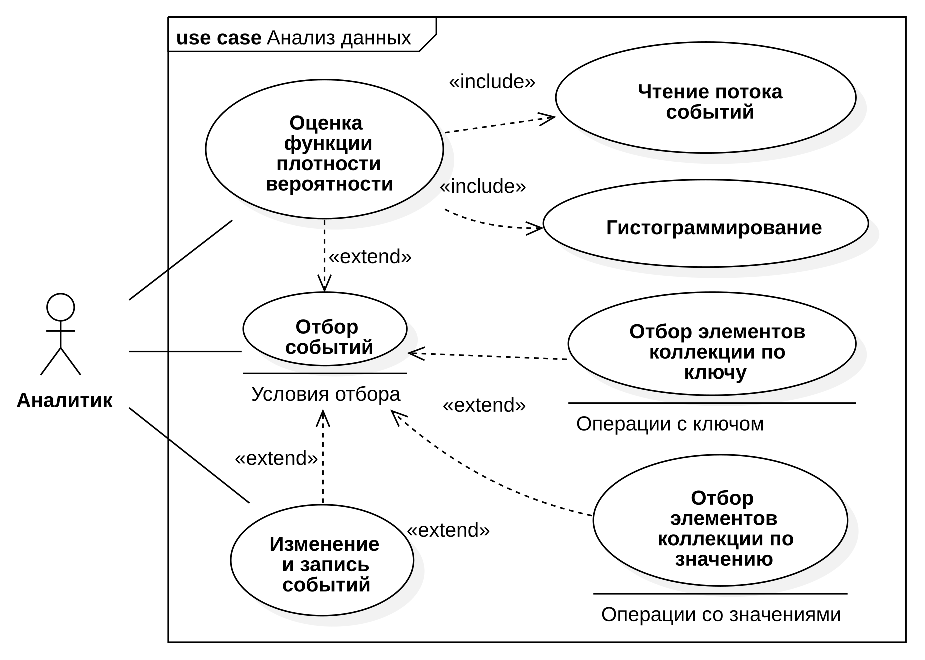
\includegraphics[width=0.85\linewidth]{images/usecases/analysis-usecase.eps}
    \caption{Диаграмма вариантов использования в сценарном контексте анализа данных}
    \label{fig:analysis-main-usecases}
\end{figure}

Для высокоуровневых сценариев отбора событий вводится точка расширения
в которой должен реализовываться отбор, в то время как логика
вычитки и обработки событий может быть реализована в обобщённой
форме. На более низком уровне, во множестве условий отбора, с технической
точки зрения необходимо различать отбор элементов коллекций по
значению и отбор по ключу, поскольку различия в реализации между этими
вариантами весьма существенны.

Главной отличительной особенностью такого контекста является требование к
\emph{детерминированности} вычисления (реконструкции) --
преобразование входных данных алгоритмом должно всегда
оставаться воспроизводимым. Иными словами, преобразование
входных данных должно быть идемпотентно.

\subsection{Сопровождение набора данных}

Другим распространённым сценарием использования программного
окружения является сопровождение эксперимента в ходе набора данных.
В данном случае речь идёт о контроле состояния детекторов и их
диагностике в режиме реального времени (онлайн-реконструкция).
Практически это реализуется посредством случайной выборки небольшой
доли событий из непрерывного потока, что позволяет получать
репрезентативную статистику в ограниченном временном окне, имеющем
фиксированную хронологическую или логическую привязку.

Ключевое отличие данного сценария от полной реконструкции заключается
в приоритете скорости обработки и устойчивости алгоритмов над
точностью и глубиной анализа. Целью становится получение быстрых,
иногда грубых оценок, достаточных для мониторинга работоспособности
установки. В этом контексте алгоритмы реконструкции реализуются в
упрощённой форме, модели заменяются правдоподобным приближением.
Для примера рассмотрим, как задачи из предыдущей группы сценариев
изменяются в рамках данного контекста:

\begin{itemize}
    \item Выделение зарядовых кластеров на выполняется без учёта
    неэффективности чувствительных элементов, рассматривается
    их упрощённая геометрия.
    \item Составление и рассмотрение треков частиц может выполняться
    на основе ограниченного набора вариантов. Например, задача поиска
    трека формулируется без учёта множественного рассеяния, с
    усреднением координат вместо комбинаторного рассмотрения для
    многослойных детекторов
    \item Модель трека аппроксимируется упрощённой функцией
    (с пропагатором прямой или винтовой линией),
    методы Рунге-Кутта не применяются для вычисления ковариации
    в магнитном поле, само поле представлено однородной аппроксимацией
    в конечном объёме
    \item Оценка энерговыделения в откликах калориметров выполняется
    на основе глобальных максимумов сигнала или интегральных сумм ,
    без учёта нелинейностей и нестационарных
    эффектов.
    \item Анализ конкурирующих гипотез может быть заменён случайным
    выбором с целью формирования усреднённой картины.
\end{itemize}

С точки зрения высокоуровневых вариантов использования, данный контекст
представляет собой подмножество контекста анализа данных,
расширенное средствами журналирования и телеметрии, как это изображено
на рисунке~\ref{fig:online-monitoring-usecases-main}.

\begin{figure}[ht!]
    \centering
    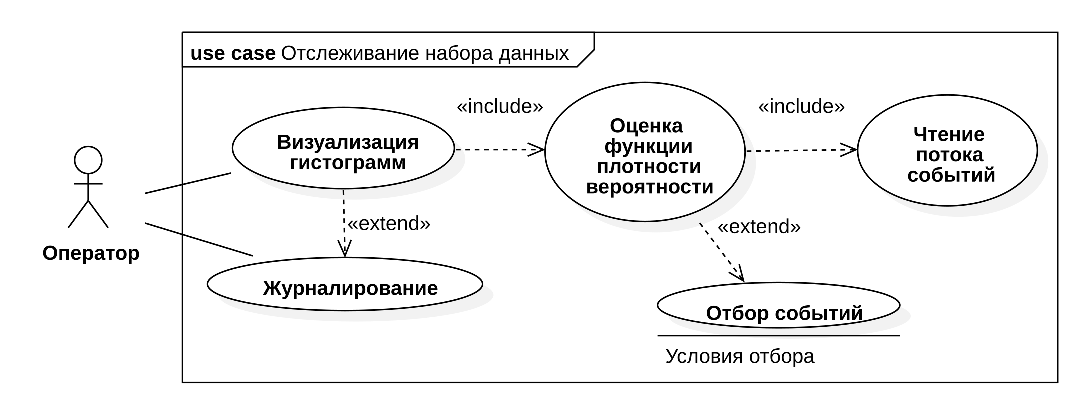
\includegraphics[width=0.95\linewidth]{images/usecases/onlineMonitoring.eps}
    \caption{Диаграмма вариантов использования в сценарном контексте сопровождения набора данных}
    \label{fig:online-monitoring-usecases-main}
\end{figure}

Требования предъявляемые к ПО в данном сценарии отличаются также
и в смысле устойчивости алгоритмов и отказоустойчивости ПО в целом.
Такое ПО предназначено для использования дежурными операторами
экспериментальной установки во время сеансов набора данных. Допустимо
снижение сценарной гибкости и статистической полноты в пользу
производительности и простоты эксплуатации. Требования
детерминированности и идемпотентности преобразований здесь
значительно слабее, чем в предыдущем контексте.

\subsection{Калибровка детекторов}

%В широком смысле калибровка детектора подразумевает отыскание аппроксимации
%\emph{функции отклика детектора}~\cite{exp-methods-Abramov1977}
%в некоторой ограниченной области. Зачастую этот сценарий требует
%получения выборки событий, отвечающей определённому критерию,
%или, напротив, -- максимального ослабления критериев отбора в
%какой-то определённой области. Так, для рассмотренных выше примеров:
В широком смысле калибровка подразумевает восстановление \emph{функции отклика детектора}~\cite{exp-methods-Abramov1977} в ограниченной области. Для этого требуется либо особая выборка событий, либо, напротив, ослабление условий отбора.
В данном контексте рассмотренные ранее примеры выражаются в следующих
сценариях:

\begin{itemize}
    \item Выделение зарядовых кластеров на микропаттерных детекторах
    обычно производится на основе характеристической диаграммы
    отношения амплитуд в области заданной
    некоторым невыпуклым многоугольником. Отыскание этого
    многоугольника представляет собой одну из задач при калибровки
    микропаттерных детекторов, для этой цели различные обрезания
    (временные и координатные) калибруемого детектора должны быть сняты.
    \item После прямых (геодезических) измерений положения детекторов проводят
    т.н. процедуру физического выравнивания (\emph{alignment})
    детекторов установки на основе реконструированной информации о
    треках, уточняя таким образом, геометрию установки, часто с точностью
    намного превышающую прямые измерения. Часто, для этого необходим
    максимально широкий пучок, засвечивающий наибольшую область
    чувствительного объёма детекторов, в широких угловых диапазонах.
    \item Задача реконструкции треков опирается на знание разрешений
    детекторов и карт их эффективности, получение которых представляет
    собой отдельную группу сценариев использования. Для этого реконструкция
    треков производится с исключённым детектором-объектом исследования.
    \item Один из вариантов калибровки калориметров состоит в отыскании
    коэффициентов пропорциональности энерговыделения регистрируемой амплитуде
    на основе известных спектров. Для этого спектры должны быть сначала
    выделены из данных, что составляет отдельную задачу анализа.
    \item Оценивание конкурирующих гипотез для калибровки нередко
    производится с ослабленными требованиями, и в этом смысле часто
    представляет собой даже более вычислительно-ёмкую задачу.
\end{itemize}

В целом, задачи калибровки детекторов во многом пересекаются с задачами
анализа, зачастую, с точки зрения сценариев использования, составляя
их подмножество, как это изображено на рисунке~\ref{fig:usecases-get-calibrations}.

\begin{figure}[ht!]
    \centering
    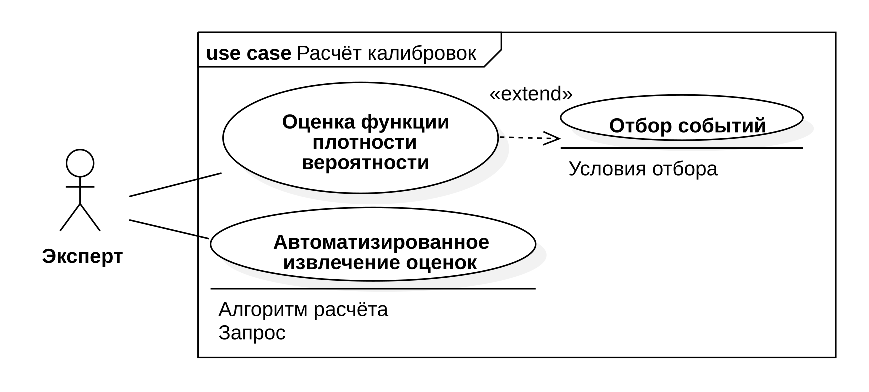
\includegraphics[width=0.75\linewidth]{images/usecases/calibration-usecase.eps}
    \caption{Диаграмма вариантов использования в сценарном контексте извлечения калибровочной информации}
    \label{fig:usecases-get-calibrations}
\end{figure}

Помимо необходимости низкоуровневого доступа к данным объектной
модели (на уровне откликов индивидуальных чувствительных элементов,
формулируемых в точке расширения <<\emph{запрос}>>),
важное прикладное значение могут иметь средства автоматизированного
извлечения информации полученной на основе функции плотности
вероятности, различных спектров и их производных значений, что
целесообразно выделить в отдельный вариант использования с соответствующей
точкой расширения (<<\emph{алгоритм расчёта}>>).

\subsection{Точки расширения на основе вариантов использования}

С точки зрения прикладного программирования, во всех перечисленных
контекстах, варианты использования имеют общие функциональные
элементы, для которых целесообразно предусмотреть обобщённые
реализации воплощающие выбранные черты архитектуры, и
предусмотреть  зависящие от конкретного эксперимента точки
расширения в которых производится реализация конкретной задачи.

\begin{itemize}
    \item  \emph{Идентификация отдельных детекторов} на различных
    логических уровнях -- от элементарных чувствительных элементов
    установки, например, ячейки калориметра, проволоки в зарядовой камере,
    стрипа в микропаттерном детекторе, до детекторных сборок, например
    модульного калориметра как целое, участка трекера вне магнитного
    поля, баррельной части установки для радиальной коллайдерной
    постановки.
    \item Работа с \emph{коллекциями} случайных величин относящихся к
    детекторам или сборкам -- итерирование, формирование выборок,
    различные свёрточные операции и агрегатные функции.
    \item Применение логических условий на случайные величины --
    логическая \emph{дискриминация} случайных величин по определённому
    признаку, выполняемая с использованием идентификаторов детекторов
    или их сборок.
    \item Функция плотности вероятности (или её аппроксимации) --
    для представления различных спектров, статистических
    перенормировок, оценки средних значений и их доверительных
    интервалов. Основным программным инструментом здесь является.
    \emph{гистограмма} (в первую очередь в смысле структуры данных,
    а не графического средства).
\end{itemize}

При этом, конкретные численные процедуры -- вроде численной аппроксимации,
решения СЛАУ, итеративной минимизации функционалов встраиваются в такую
парадигму как отдельные элементы.

Номенклатура детекторов и логическая топология определяются
конкретной установкой, иерархией её узлов и подсистем. Важно, что
объектная модель события во многом подчинена этой иерархии:
оцифрованные сигналы от отдельных чувствительных элементов
объединяются в рамках коллекций в сущности, соответствующие
физическим понятиям (зарядовый кластер, ливень в калориметре,
трек), логически отвечающие отдельным детекторам (станция трекера,
модуль калориметра, трекер). Попытка обобщить эти отношения в рамках
какой-нибудь одной системы скорее всего будет создавать больше сложностей
чем решать.

По этой причине, номенклатура детекторов и объектная модель должны
быть вынесены в точки расширения, в то время как коллекции и операции над
ними, включая логическую дискриминацию, целесообразно объединить в
рамках обобщённых алгоритмов, задающих инварианты системы.
